\documentclass[../../main.tex]{subfiles}
\begin{document}

{\bf [解]}

$C\Bigl(c, \dfrac{1}{c}\Bigr)$ ($c > 0$) での $y = \dfrac{1}{x}$ の接線$\ell$は
\begin{align}
  \ell: y = -\dfrac{1}{c^2} x + \dfrac{2}{c}
\end{align}
であるから，これと $x, y$ 軸の交点は各々 $P(2c, 0)$，$Q\Bigl(0, \dfrac{2}{c}\Bigr)$ である．

\begin{figure}[htb]
  \centering
  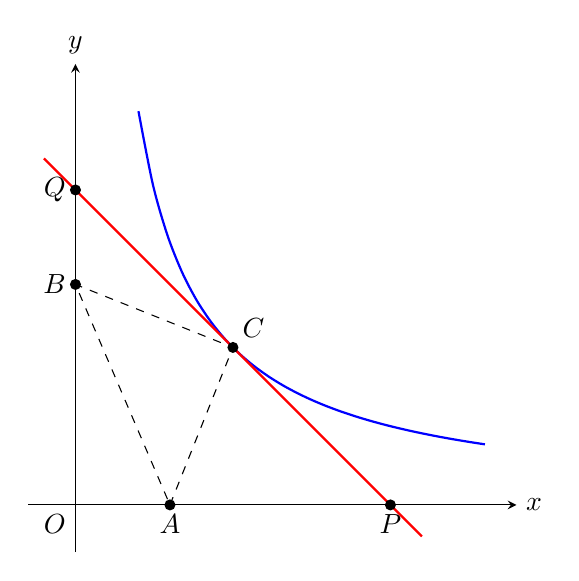
\begin{tikzpicture}[scale=2, >=stealth]
    \draw[->] (-0.3,0) -- (2.8,0) node[right] {$x$};
    \draw[->] (0,-0.3) -- (0,2.8) node[above] {$y$};
    \node[below left] at (0,0) {$O$};
    \draw[domain=0.4:2.6, smooth, variable=\x, thick, blue] plot ({\x}, {1/\x});
    % Tangent line at c=1: y = -x + 2
    \draw[thick, red] (-0.2, 2.2) -- (2.2, -0.2);
    \fill (1,1) circle (1pt) node[above right] {$C$};
    \fill (2,0) circle (1pt) node[below] {$P$};
    \fill (0,2) circle (1pt) node[left] {$Q$};
    \fill (0.6,0) circle (1pt) node[below] {$A$};
    \fill (0,1.4) circle (1pt) node[left] {$B$};
    \draw[dashed] (0.6,0) -- (1,1) -- (0,1.4) -- cycle;
  \end{tikzpicture}
  \caption{接線と $x,y$ 軸の交点，最大面積を与える $\triangle ABC$ の配置}
\end{figure}

題意の条件より，$\triangle ABC$ が $D$ の内部にあるので，線分$AC, BC$が$xy \le 1$にあるためには$A,B$がそれぞれ$P,Q$よりも原点に近い位置にあれば良いから
\begin{align}
  \begin{cases}
    0 \le a \le 2c \\
    0 \le b \le \dfrac{2}{c}
  \end{cases} \label{eq:1}
\end{align}
である．このもとで三角形$ABC$の面積$S$の最大値を考える．
$S$は三角形の面積公式から
\begin{align}
  S = \dfrac{1}{2} \Bigl| b(c - a) + \dfrac{a}{c} \Bigr| \equiv \dfrac{|f(a,b,c)|}{2}
\end{align}
である．$a, c$ を固定して$f(a,b,c)$の最大値を考える．

\subparagraph{$1^\circ$ $c - a = 0$ の時}

この時は$f(a,b,c)=\dfrac{a}{c}$だから
\begin{align}
  S = \dfrac{1}{2} \dfrac{a}{c} \quad (\because a, c > 0) = \dfrac{1}{2} \label{eq:2}
\end{align}
である．ただし最後の等号で場合分けの条件$a=c$を用いた．

\subparagraph{$2^\circ$ $c - a \ne 0$ の時}

この時は$f(a,b,c)$は $b$ の単調関数なので，\cref{eq:1}より$S$ は 端点 $b = 0$ または $b = \dfrac{2}{c}$ の時に最大となる．よって
\begin{align}
  \max S = \max \Bigl\{ \dfrac{1}{2} \dfrac{a}{c}, \,\, \dfrac{1}{2}\Bigl|2 - \dfrac{a}{c}\Bigr| \Bigr\}
\end{align}
である．\cref{eq:1}より$0\le\dfrac{a}{c}\le 2$だから絶対値を外して
\begin{align}
  \max S = \max \Bigl\{ \dfrac{1}{2} \dfrac{a}{c}, \,\, \dfrac{1}{2}\left(2 - \dfrac{a}{c}\right) \Bigr\} \label{eq:3}
\end{align}
である．
\casesend

以上\cref{eq:2,eq:3}をまとめて
\begin{align}
  S &=
  \begin{cases}
    \dfrac{1}{2} & \left(a = c \right) \\
    \max \Bigl\{ \dfrac{1}{2} \dfrac{a}{c}, \,\, \dfrac{1}{2}\left(2 - \dfrac{a}{c}\right) \Bigr\} & \left(a \neq c\right)
  \end{cases} \label{eq:4}
\end{align}
である．
そこで次に $a,c$ を\cref{eq:1}の範囲，すなわち $0 \le \dfrac{a}{c} \le 2$ で動かす．$y=\dfrac{a}{2c}, y=\dfrac{1}{2}\left(2-\dfrac{c}{a}\right)$を$t=a/c$を横軸にしてグラフに示すと以下のようになる．

\begin{figure}[htb]
  \centering
  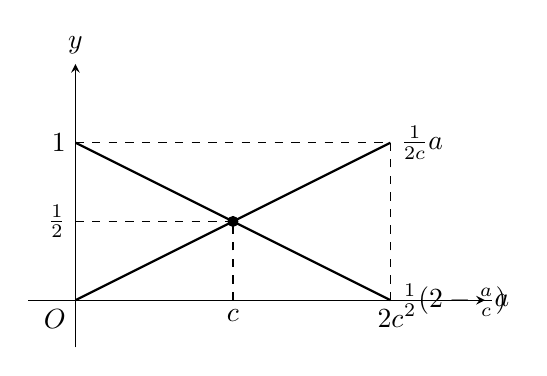
\begin{tikzpicture}[scale=2, >=stealth]
    \draw[->] (-0.3,0) -- (2.6,0) node[right] {$a$};
    \draw[->] (0,-0.3) -- (0,1.5) node[above] {$y$};
    \node[below left] at (0,0) {$O$};
    \draw[thick] (0,0) -- (2,1) node[right] {$\frac{1}{2c}a$};
    \draw[thick] (0,1) -- (2,0) node[right] {$\frac{1}{2}(2-\frac{a}{c})$};
    \draw[dashed] (1,0) node[below] {$c$} -- (1,0.5);
    \draw[dashed] (0,0.5) node[left] {$\frac{1}{2}$} -- (1,0.5);
    \fill (1,0.5) circle (1pt);
    \draw[dashed] (2,0) node[below] {$2c$} -- (2,1);
    \draw[dashed] (0,1) node[left] {$1$} -- (2,1);
  \end{tikzpicture}
  \caption{$S$の最大値を与える$a/c$の様子}
\end{figure}

従って，グラフより$S$の最大値は$a=0,2c$の時の$\max S=1$である．対応する$b$を\cref{eq:3}から考えて$(a,b)=(0,2/c),(2c,0)$である．この時の$\triangle ABC$の様子は下図のようになる．これはそれぞれ$BC, CA$が$y=1/x$の接線と一致する時である．

\begin{figure}[htb]
  \centering
  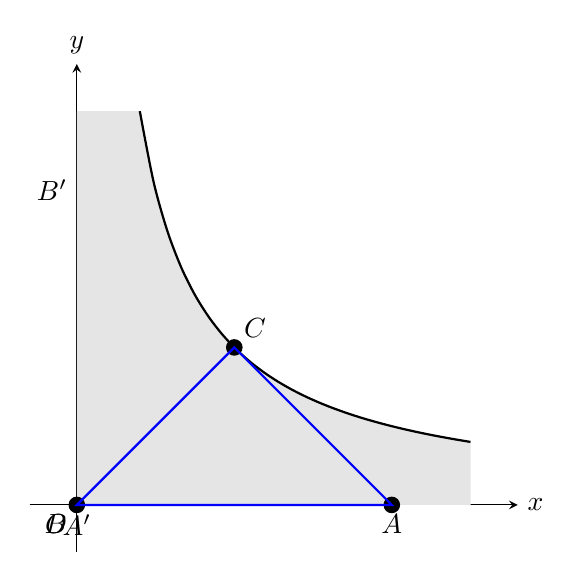
\begin{tikzpicture}[scale=2, >=stealth]
    \draw[->] (-0.3,0) -- (2.8,0) node[right] {$x$};
    \draw[->] (0,-0.3) -- (0,2.8) node[above] {$y$};
    \node[below left] at (0,0) {$O$};
    % Shaded Region D
    \begin{scope}
      \clip (0,0) -- (2.5,0) -- (2.5,2.5) -- (0,2.5) -- cycle;
      \fill[gray!20] (0,0) -- (0,2.5) -- plot[domain=0.4:2.5, smooth] ({\x},{1/\x}) -- (2.5,0) -- cycle;
    \end{scope}
    \draw[domain=0.4:2.5, smooth, variable=\x, thick] plot ({\x}, {1/\x});
    \fill (1,1) circle (1.5pt) node[above right] {$C$};
    \fill (2,0) circle (1.5pt) node[below] {$A$};
    \fill (0,0) circle (1.5pt) node[below left] {$B$};
    \draw[thick, blue] (2,0) -- (0,0) -- (1,1) -- cycle;
    \node[left] at (0,2) {$B'$};
    \node[below] at (0,0) {$A'$};
  \end{tikzpicture}
  \caption{最大面積を与える $\triangle ABC$ の配置}
\end{figure}

\end{document}
